Diffie–Hellman key exchange [\cite{li2010research}] is a method of securely exchanging cryptographic keys over a public channel
and was one of the first public-key protocols
as conceived by Ralph Merkle and named after Whitefield Diffie and Martin Hellman.
DH is one of the earliest practical examples of public key exchange implemented within the field of cryptography.
Published in 1976 by Diffie and Hellman, this is the earliest publicly known work that proposed the idea of a private
key and a corresponding public key.
Traditionally, secure encrypted communication between two parties required that they first exchange keys by some secure physical means,
such as paper key lists transported by a trusted courier.
The Diffie–Hellman key exchange method allows two parties that have no prior knowledge of
each other to jointly establish a shared secret key over an insecure channel.
This key can then be used to encrypt subsequent communications using a symmetric-key cipher.
Although Diffie–Hellman key agreement itself is a non-authenticated key-agreement protocol, it provides the basis for a
variety of authenticated protocols, and is used to provide forward secrecy in Transport Layer Security's ephemeral modes
(referred to as EDH or DHE depending on the cipher suite).

\subsection{Description}\label{subsec:description}
Diffie–Hellman key exchange establishes a shared secret between two parties that can be used for secret communication
for exchanging data over a public network.
An analogy illustrates the concept of public key exchange by using colors instead of very large numbers:
\begin{figure}[H]
    \centering
    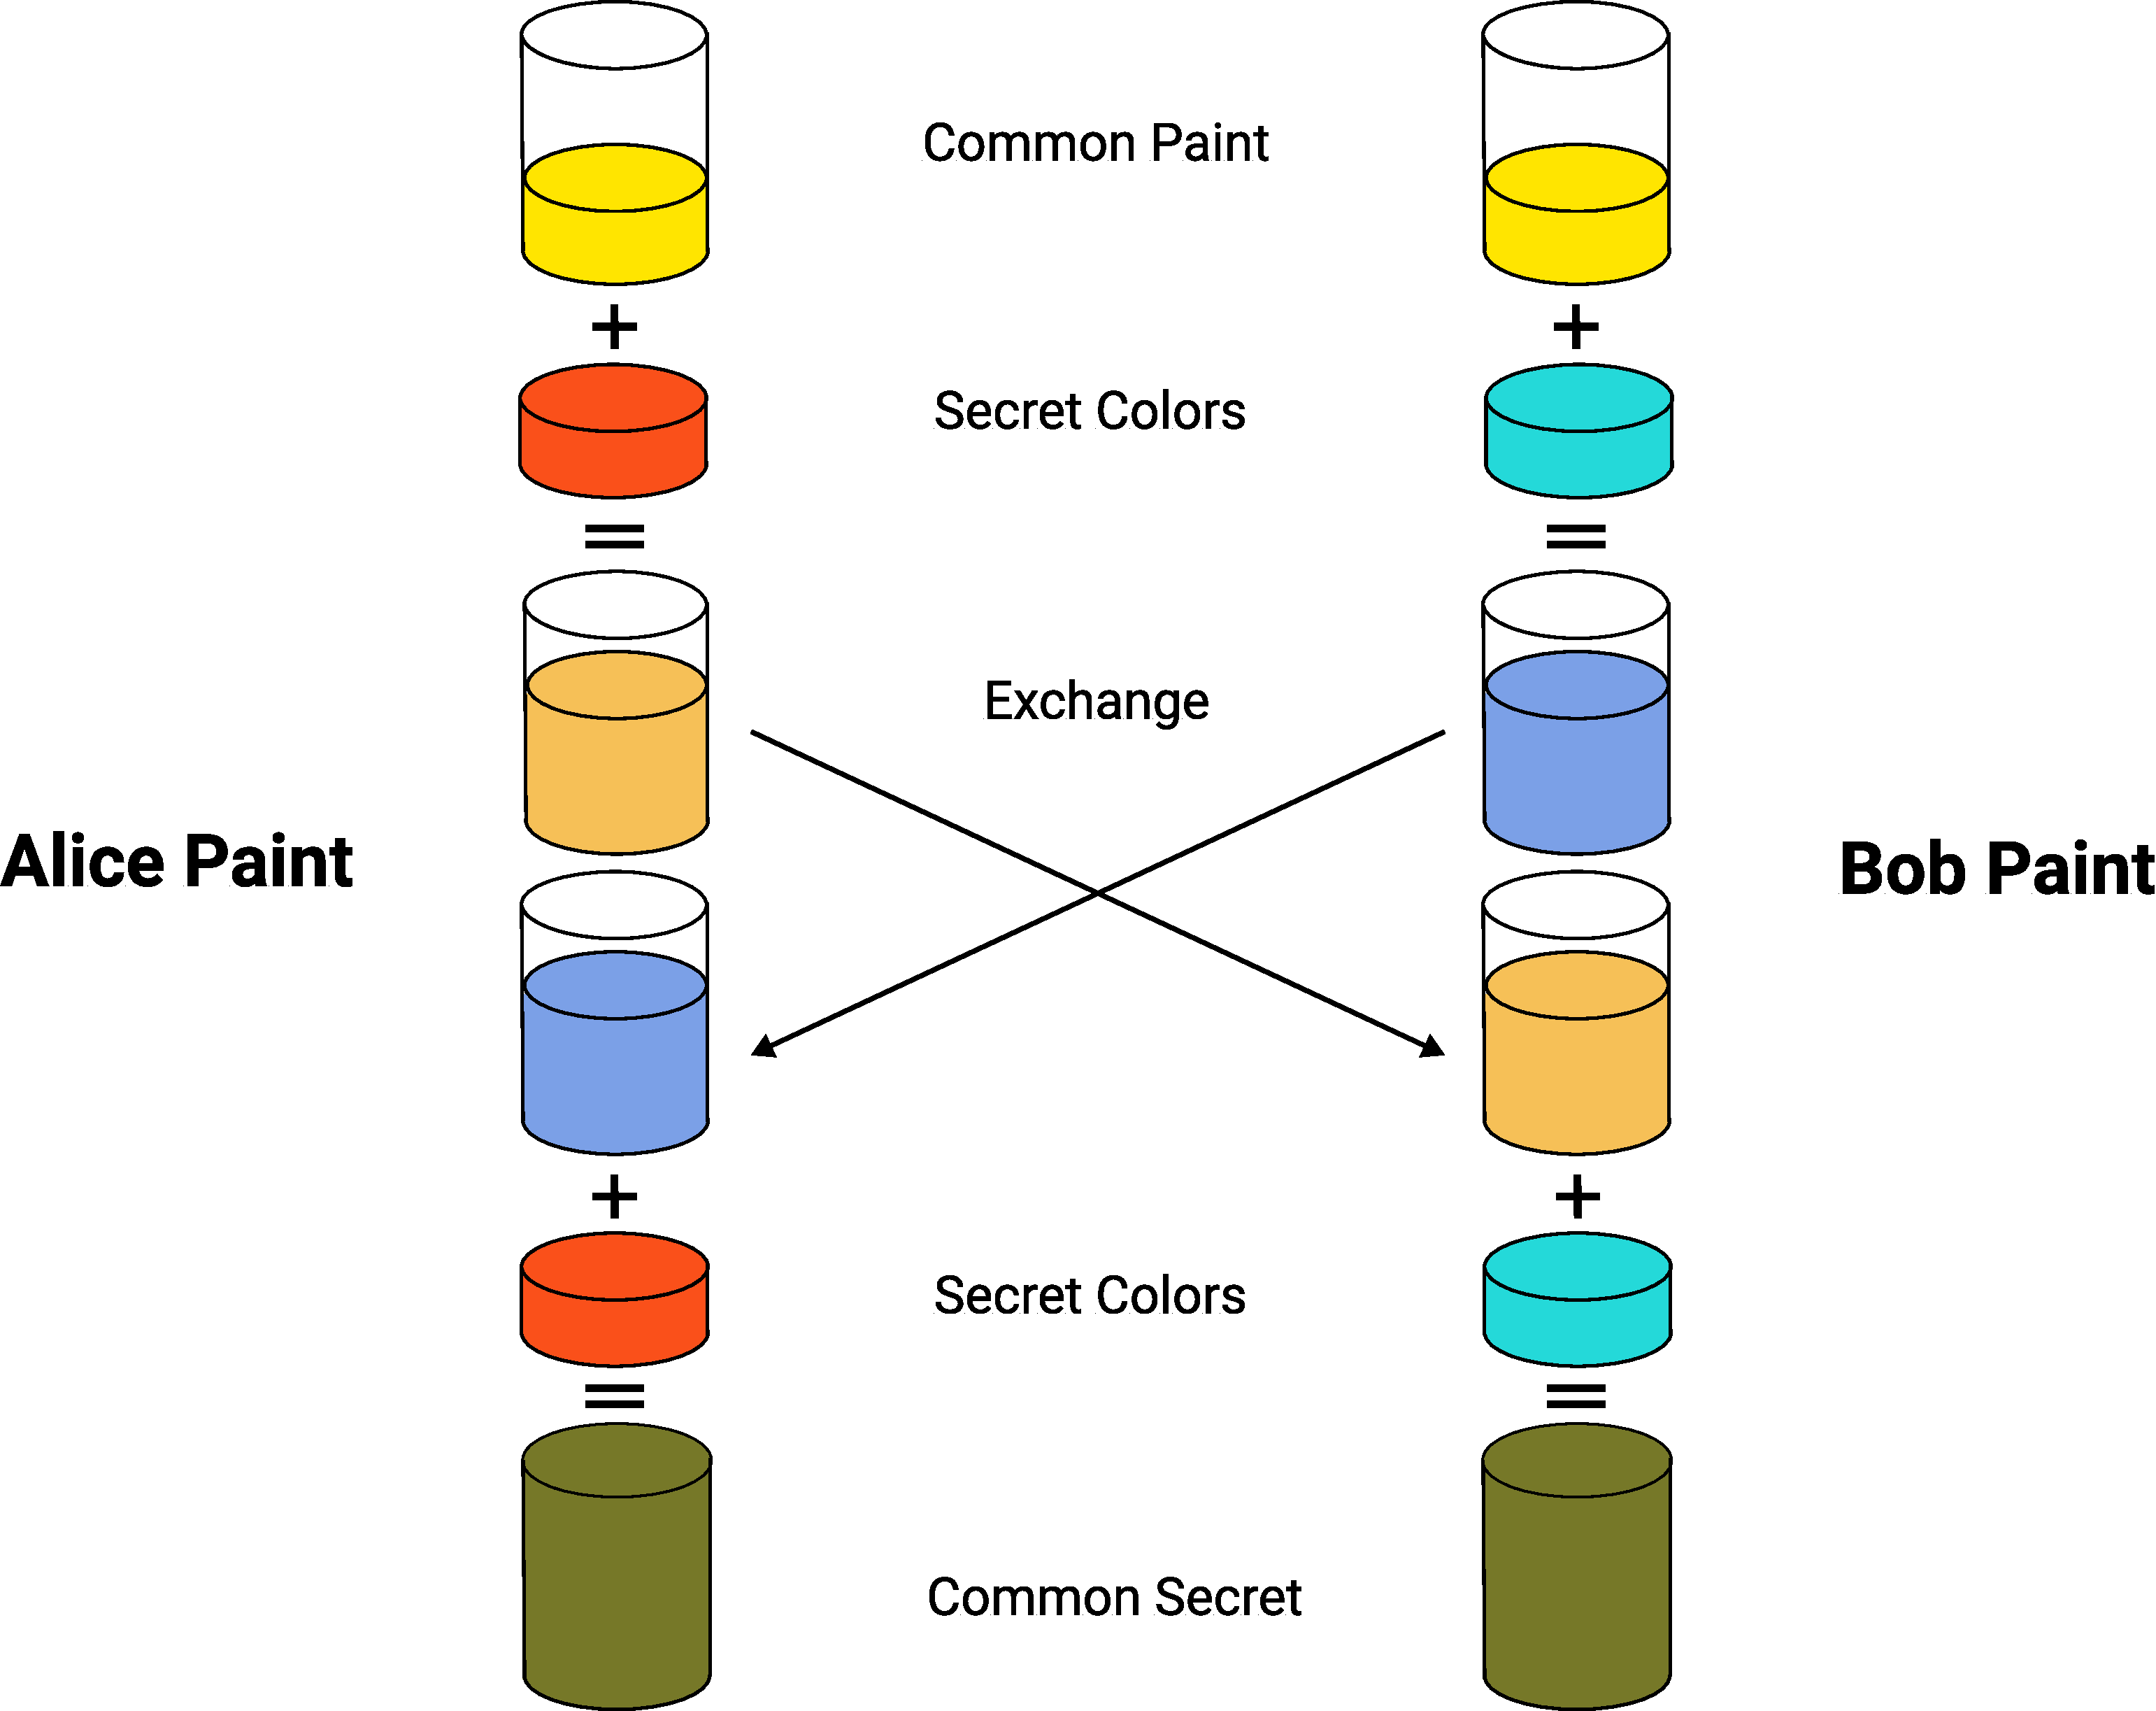
\includegraphics[width=1\textwidth]{Pictures/Diffie-Hellman.pdf}
    \caption{Illustration of the concept behind Diffie–Hellman key exchange. Source: }\label{fig:figure4}
\end{figure}
The process begins by having the two parties, Alice and Bob, publicly agree on an arbitrary starting color that does
not need to be kept secret (but should be different every time).
In this example, the color is yellow.
Each person also selects a secret color that they keep to themselves – in this case, red and blue-green.
The crucial part of the process is that Alice and Bob each mix their own secret color together with their mutually
shared color, resulting in orange-tan and light-blue mixtures respectively, and then publicly exchange the two mixed colors.
Finally, each of them mixes the color they received from the partner with their own private color.
The result is a final color mixture (yellow-brown in this case) that is identical to the partner's final color mixture.
If a third party listened to the exchange, it would only know the common color (yellow) and the first mixed colors
(orange-tan and light-blue), but it would be difficult for this party to determine the final secret color (yellow-brown).
Bringing the analogy back to a real-life exchange using large numbers rather than colors, this determination is
computationally expensive.
It is impossible to compute in a practical amount of time even for modern supercomputers.

\subsection{Cryptographic explanation}\label{subsec:cryptographic-explanation}
The simplest and the original implementation of the protocol uses the multiplicative group of integers modulo $p$,
where $p$ is prime, and $g$ is a primitive root modulo $p$.
These two values are chosen in this way to ensure that the resulting shared secret can take on any value from $1$ to $p-1$.
Here is an example of the protocol, with non-secret values in \textcolor{blue}{blue}, and secret values in \textcolor{red}{red}.
\begin{enumerate}
    \item Alice and Bob publicly agree to use a modulus $\textcolor{blue}{p = 23}$ and base
    $\textcolor{blue}{g = 5}$, which is a primitive root modulo 23.
    \item Alice chooses a secret integer $\textcolor{red}{a} = 4$, then sends the
    Bob $\textcolor{blue}{A} = \textcolor{blue}{g}^{\textcolor{red}{a}} \, mod  \, \textcolor{blue}{p}$
    \[
        \textcolor{blue}{A} = \textcolor{blue}{5}^{\textcolor{red}{4}} \, mod  \, \textcolor{blue}{23} = \textcolor{blue}{4}
    \]
    \item Bob chooses a secret integer $\textcolor{red}{b} = 3$,
    then sends Alice $\textcolor{blue}{B} = \textcolor{blue}{g}^{\textcolor{red}{b}} \, mod  \, \textcolor{blue}{p}$
    \[
        \textcolor{blue}{B} = \textcolor{blue}{5}^{\textcolor{red}{3}} \, mod  \, \textcolor{blue}{23} = \textcolor{blue}{10}
    \]

    \item Alice computes $\textcolor{red}{s} = \textcolor{blue}{B}^{\textcolor{red}{a}} \, mod \, p$
    \[
        \textcolor{red}{s} = \textcolor{blue}{10}^{\textcolor{red}{4}} \, mod \, \textcolor{blue}{23} = \textcolor{red}{18}
    \]
    \item Bob computes $\textcolor{red}{s} = \textcolor{blue}{A}^{\textcolor{red}{b}} \, mod \, p$
    \[
        \textcolor{red}{s} = \textcolor{blue}{4}^{\textcolor{red}{3}} \, mod \, \textcolor{blue}{23} = \textcolor{red}{18}
    \]
    \item Alice and Bob now share a secret, the number $18$.
\end{enumerate}
Both Alice and Bob have arrived at the same values because under mod $p$:
\[
    \textcolor{blue}{A}^{\textcolor{red}{b}} \, mod \, \textcolor{blue}{p}
    = \textcolor{blue}{g}^{\textcolor{red}{ab}} \, mod \, \textcolor{blue}{p}
    = \textcolor{blue}{g}^{\textcolor{red}{ba}} \, mod \, \textcolor{blue}{p}
    = \textcolor{blue}{B}^{\textcolor{red}{a}} \, mod \, \textcolor{blue}{p}
\]
More specifically,
\[
    (\textcolor{blue}{g}^{\textcolor{red}{a}} \, mod \, \textcolor{blue}{p})^{\textcolor{red}{b}} \, mod \, \textcolor{blue}{p}
    = (\textcolor{blue}{g}^{\textcolor{red}{b}} \, mod \, \textcolor{blue}{p})^{\textcolor{red}{a}}
\]
Only $a$ and $b$ are kept secret.
All the other values: $p$, $g$, $ga \; mod \; p$, and $gb\; mod \; p$ are sent in the clear.
The strength of the scheme comes from the fact that $gab \; mod \; p = gba \; mod \; p$ take extremely long times to compute by any
known algorithm just from the knowledge of $p, g, ga \; mod \; p$, and $gb \; mod \; p$.
Once Alice and Bob compute the shared secret they can use it as an encryption key, known only to them, for sending
messages across the same open communications channel.
Of course, much larger values of $a, b$, and $p$ would be needed to make this example secure, since there are only $23$ possible
results of $n \; mod \; 23$.
However, if $p$ is a prime of at least 600 digits, then even the fastest modern computers using the fastest known algorithm
cannot find a given only $p, g, ga \; mod \; p$, and $gb \; mod \; p$.
Such a problem is called the discrete logarithm problem [\cite{mccurley1990discrete}].
The computation of $ga \; mod \; p$ is known as modular exponentiation and can be done efficiently even for large numbers.
Note that $g$ need not be large at all, and in practice is usually a small integer, like $2, 3, \cdots$.

\subsection{Secrecy Chart}\label{subsec:secrecy-chart}
The chart below depicts who knows what, again with non-secret values in \textcolor{blue}{blue}, and secret values in \textcolor{red}{red}.
Here Eve is an eavesdropper – she watches what is sent between Alice and Bob, but she does not alter the contents of their communications.
\begin{itemize}
    \item \textcolor{blue}{g} = public (prime) base, known to Alice, Bob, and Eve. $\textcolor{blue}{g = 5}$
    \item \textcolor{blue}{p} = public (prime) modulus, known to Alice, Bob, and Eve. $\textcolor{blue}{p = 23}$
    \item \textcolor{red}{a} = Alice's private key, known only to Alice. $\textcolor{red}{a = 6}$
    \item \textcolor{red}{b} = Bob's private key known only to Bob. $\textcolor{red}{b = 15}$
    \item \textcolor{blue}{A} = Alice's public key, known to Alice, Bob, and Eve. $\textcolor{blue}{A = g}^{\textcolor{red}{a}} \, mod \, \textcolor{blue}{p = 8}$
    \item \textcolor{blue}{B} = Bob's public key, known to Alice, Bob, and Eve. $\textcolor{blue}{B = g}^{\textcolor{red}{a}} \, mod \, \textcolor{blue}{p = 8}$
\end{itemize}
\begin{center}
    \begin{table}
        \begin{tabular}{|c|c|c|c|c|c|}
            \hline
            \multicolumn{2}{|c|}{Alice} & \multicolumn{2}{c|}{Bob} & \multicolumn{2}{c|}{Eve}
            \cr \hline
            known & unknown & known & unknown & known & unknown
            \cr \hline
            $\textcolor{blue}{p = 23}$ & & $\textcolor{blue}{p = 23}$  & & $\textcolor{blue}{p = 23}$ &
            \cr \hline
            $\textcolor{blue}{g = 5}$ & & $\textcolor{blue}{g = 5}$ & & $\textcolor{blue}{g = 5}$ &
            \cr \hline
            $\textcolor{red}{a = 6}$ & $\textcolor{red}{b}$ & $\textcolor{red}{b = 15}$ & $\textcolor{red}{a}$ & & $\textcolor{red}{a, b}$
            \cr \hline
            $\textcolor{blue}{A = 5}^{\textcolor{red}{a}} \, mod \, \textcolor{blue}{23}$ & & $\textcolor{blue}{B = 5}^{\textcolor{red}{b}} \, mod \, \textcolor{blue}{23}$ & & &
            \cr \hline
            $\textcolor{blue}{A = 5}^{\textcolor{red}{6}} \, mod \, \textcolor{blue}{23} = \textcolor{blue}{8}$ & & $\textcolor{blue}{B = 5}^{\textcolor{red}{15}} \, mod \, \textcolor{blue}{23} = \textcolor{blue}{19}$ & & &
            \cr \hline
            $\textbf{\textcolor{blue}{B}} = \textbf{\textcolor{blue}{19}}$ & & $\textbf{\textcolor{blue}{A}} = \textbf{\textcolor{blue}{8}}$ & & $\textcolor{blue}{A} = \textcolor{blue}{8}$, $\textcolor{blue}{B} = \textcolor{blue}{19}$ &
            \cr \hline
            $\textbf{\textcolor{red}{s}} = \textcolor{blue}{B}^{\textcolor{red}{a}} \, mod \, \textcolor{blue}{23}$ & & $\textbf{\textcolor{red}{s}} = \textcolor{blue}{A}^{\textcolor{red}{b}} \, mod \, \textcolor{blue}{23}$ & & &
            \cr \hline
            $\textbf{\textcolor{red}{s}} = \textcolor{blue}{19}^{\textcolor{red}{6}} \, mod \, \textcolor{blue}{23} = \textcolor{red}{2}$ & & $\textbf{\textcolor{red}{s}} = \textcolor{blue}{A}^{\textcolor{red}{b}} \, mod \, \textcolor{blue}{23} = \textcolor{red}{2}$ & & &
            \cr \hline

        \end{tabular}
        \label{tab:table}
    \end{table}
\end{center}
Now \textcolor{red}{s} is the shared secret key and it is known to both Alice and Bob, but not to Eve.
Note that it is not helpful for Eve to compute \textcolor{blue}{AB}, which equals
$\textcolor{blue}{g}^{\textcolor{red}{a} + \textcolor{red}{b}} \, mod \, \textcolor{blue}{p}$.
Note that it should be difficult for Alice to solve for Bob's private key or for Bob to solve for Alice's private key.
If it is not difficult for Alice to solve for Bob's private key (or vice versa), Eve may simply substitute her own
private / public key pair, plug Bob's public key into her private key, produce a fake shared secret key, and solve for
Bob's private key (and use that to solve for the shared secret key.
Eve may attempt to choose a public / private key pair that will make it easy for her to solve for Bob's private key).

\subsection{Implementation}\label{subsec:implementation}
\begin{figure}[H]
    \centering
    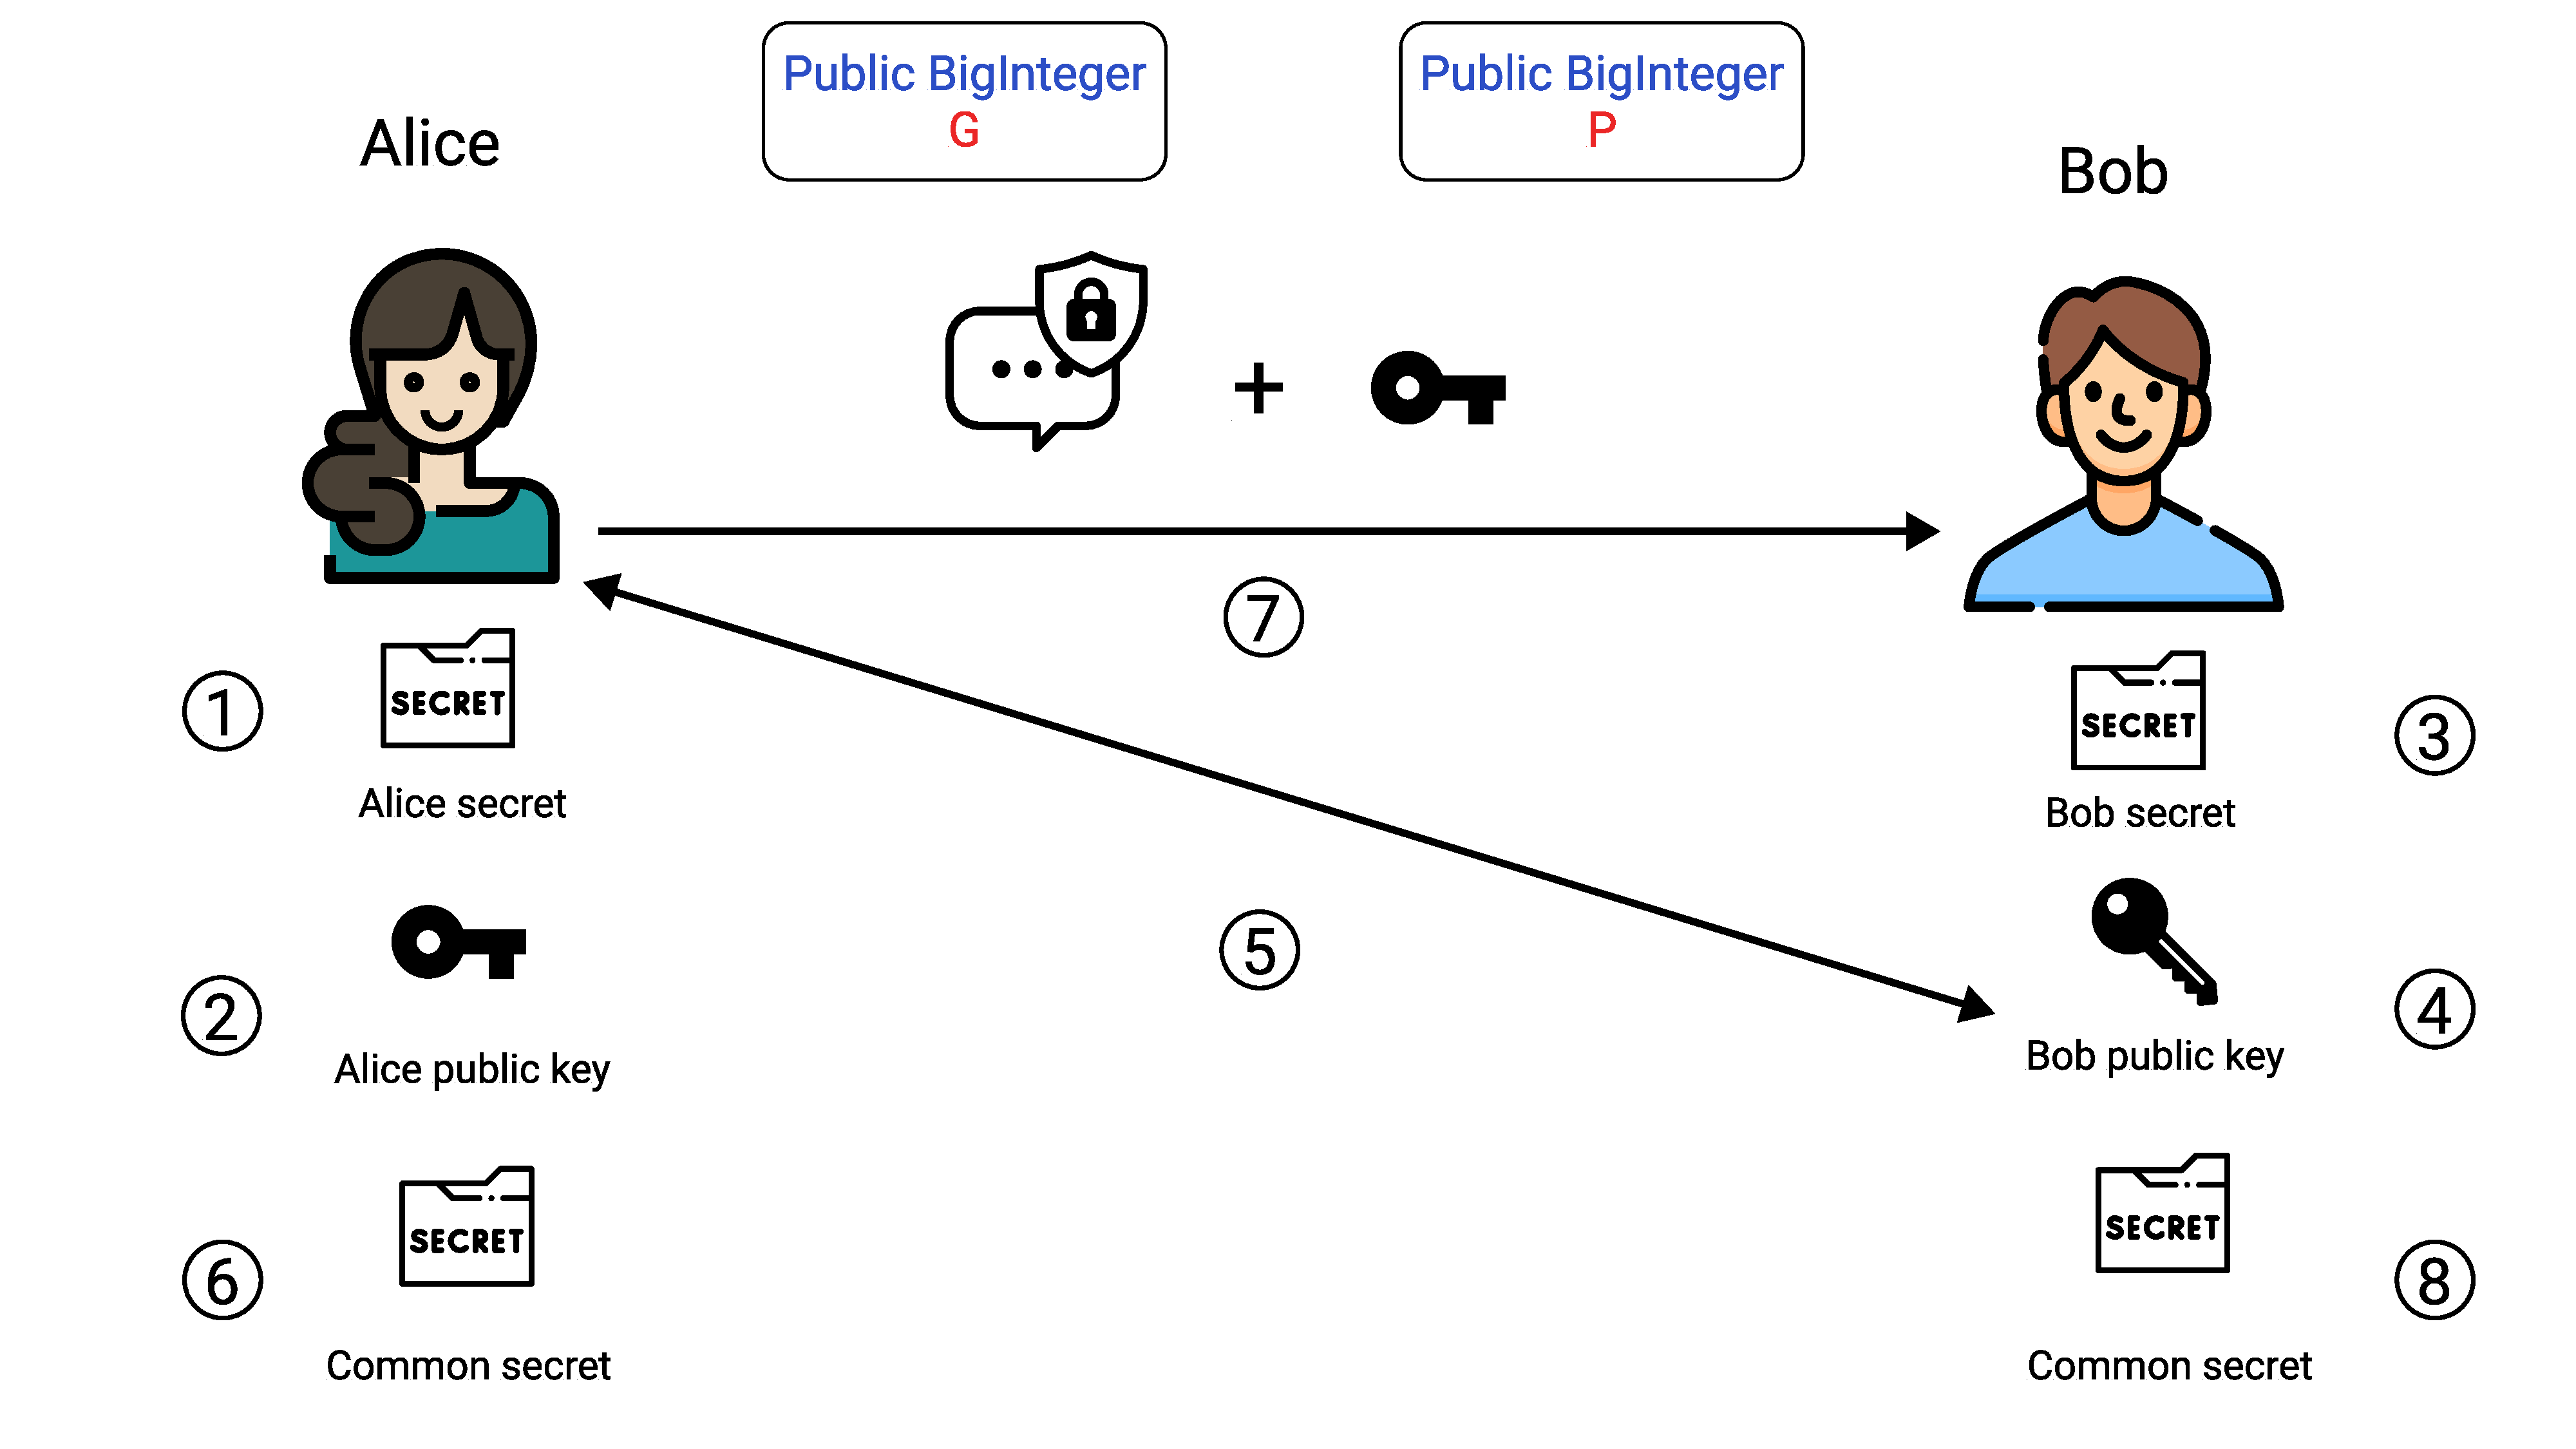
\includegraphics[width=1\textwidth]{Pictures/Key_Exchange}
    \caption{Secret chat encryption concept diagram. Source: }\label{fig:figure7}
\end{figure}
Assume that Alice wants to write a secret message to the Bob.
The secret chat encryption implemented as follows
\begin{enumerate}
    \item Given two public constants of type BigInteger: $P, G$.
    \item Alice generates a secret: Alice secret $a$, Prime BigInteger.
    \item Alice generates public key $A$ as $A=G^a \bmod P$ and stores it to database.
    \item Bob generates a secret: Bob secret $b$, Prime BigInteger.
    \item Bob generates public key $B$ as $B=G^b \bmod P$ and stores it to database.
    \item Alice reads Bob's public key $B$.
    \item Alice calculates Common secret $S$ as $S = B^a \bmod P$.
    \item Alice symmetrically encrypts message using Common secret and sends it to Bob among with her public key $A$.
    \item Bob calculates Common secret $S$ as $S = A^b \bmod P$ and decrypts message from Alice.
\end{enumerate}